%\subsection{Implementation: what can be done in practise?}


\subsection{The FloPoCo Framework: computing just right}
	\begin{frame}
		\frametitle{The FloPoCo Framework: computing just right}
		FloPoCo:\\
			\begin{itemize}
				\item C++ framework
				\item Target: FPGAs
				\item Work: generating arithmetical cores in VHDL computing just right
				\item Reference: \url{http://flopoco.gforge.inria.fr/}
			\end{itemize}
	\end{frame}

\subsection{Basic block: SOPC}
\begin{frame}
	\frametitle{Basic block: SOPC}
%\begin{multicols}{2}
%\begin{figure}[]
%  \begin{tikzpicture}[scale=0.6,every node/.style={scale=0.6}]
%    \footnotesize 
%    \node at (-1em,0)  {$x_i=$} ;
%    \foreach \x in {1,...,18} {
%%    \draw[] ($(-5*\x ex, -7ex)$) -- ($(-5*\x ex, -5ex)$) node[above] {$2^\x$} ;
%      \node (n) at ($(3.4*\x ex, 0ex)$)  {$b_{\x}$} ;
%      \draw[black!25, very thin] ($(n)+(1.7ex,1.5ex)$) -- ++(0, -3ex);
%    }
%    \node[draw, thick, rectangle, minimum width = 3.4*6ex, minimum height=3ex] (d1) at (3.4*3ex+1.7ex,0) {} ;
%    \node[hwblock, minimum width=20ex,minimum height=6ex] (T1) at ($(d1)+(0,-10ex)$) { $T_{i1}: \circ_p(c_i\times d_{i1})$};
%    \draw[hwbus,->] (d1.south) --  (T1.north) node[midway,right] {$d_{i1}$};
%
%    \node[draw, thick, rectangle, minimum width = 3.4*6ex, minimum height=3ex] (d2) at (3.4*9ex+1.7ex,0) {} ;
%    \node[hwblock, minimum width=15ex] (T2) at ($(d2)+(0,-10ex)$) { $T_{i2}$};
%    \draw[hwbus,->] (d2.south) --  (T2.north) node[midway,right] {$d_{i2}$};
%
%    \node[draw, thick, rectangle, minimum width = 3.4*6ex, minimum height=3ex] (d3) at (3.4*15ex+1.7ex,0) {} ;
%    \node[hwblock, minimum width=10ex,minimum height=3.5ex] (T3) at ($(d3)+(0,-10ex)$) { $T_{i3}$};
%    \draw[hwbus,->] (d3.south) --  (T3.north) node[midway,right] {$d_{i3}$};
%
%    
%    \node[hwblock, minimum width=50ex] (sum) at ($(T2)+(0,-11.3ex)$) {\Large $+$};
%    \draw[hwbus,->]  (T1.south) --  ($(sum.80)!(T1)!(sum.north)$) % This means: point that is the projection of T1 on the line  (sum.80) -- (sum.north)
%       node[near start] {$/$} node[near start,left] {$q_i+g$}          node[near end,right] {$\widetilde{t}_{i1}$};
%    \draw[hwbus,->]  (T2.south) --  ($(sum.80)!(T2)!(sum.north)$) node[near start] {$/$} node[near start,left] {$q_i-\alpha+g$}   node[near end,right] {$\widetilde{t}_{i2}$};
%    \draw[hwbus,->]  (T3.south) -- ($(sum.80)!(T3)!(sum.north)$) node[near start] {$/$} node[near start,left] {$q_i-2\alpha+g$}  node[near end,right] {$\widetilde{t}_{i3}$};
%
%    \draw[hwbus,->] (sum.south) --  ++(0,-6ex) node[near start] {$/$} node[near start,left] {$q_i+g$} node[near end,right] {$\widetilde{p}_i\approx c_ix_i$};
% \end{tikzpicture}
%\caption{The FixRealKCM method when $x_i$ is split in 3 chunks   \label{fig:FixRealKCM}}
%\end{figure}

\begin{figure}
  \begin{tikzpicture}[scale=1.0, every node/.style={scale=1.0}]
    \footnotesize 
     \draw[green, fill=green!20] (-0.5cm,-1.8cm) rectangle +(10cm,4.0cm);   
	 \node[green!50!black] at(0cm, -1.6cm) {SOPC};
    
    \node[hwblock, align=center,minimum width=60ex] (sum) at ($(32ex,-5ex)$) {Bit-heap based \\ summation architecture};

    \foreach \i in {0,...,3} {
      \node (x) at  ($(15*\i ex+10ex, 18ex)$) {$x_\i$};
      \coordinate (xb) at  ($(x)+(0, -3ex)$);
      \draw[hwbus,very thick] (x) --  (xb);
      
      \foreach \k in {1,...,3} {
        \node[hwblock, minimum width=5ex] (T) at ($(15*\i ex+4.5*\k ex,7ex-1*\k ex)$) { $T_{\i\k}$};
        \draw[hwbus,thick,<-]  (T.north) -- ++(0,+4ex) node [midway] {/}node [midway,right] {$\alpha$} -- (xb);
        \draw[hwbus,->] (T.south) --  ($(sum.north)!(T)!(sum.80)$);
      }
    }

    \draw[hwbus,->] (sum.south) --  ++(0,-12ex) node[near start, yshift=-6mm] {$/$} node[near start,left, yshift=-6mm] {\normalsize ($msb_{out}-lsb_{out}$)} node[near end,right] {$y$};
 \end{tikzpicture}
\end{figure}
\centering
SOPC architecture
%\end{multicols}

	\end{frame}


\subsection{Architecture generation}
\begin{frame}
	\frametitle{Architecture generation algorithm}
	\begin{algorithm}[H]
	\caption{Architecture Generation Algorithm}
	Assuming all the MSBs and LSBs are known. \\
	%computeMSBSLSBS($[msbs,lsbs][][]$) \\%//get the matrix of msbs lsbs. \\
	\For{i=1; i=Z.nbLines(); i++} {
	 	row[ ]= Z[i][ ] //pick first row of Z \\
	 	\For {j=1; j=1; j=Z.nbCols() j++} {
	 		assign(SOPC[i], row[j], {"T","X","Y"},[msbs,lsbs][i][j])
	 	}
		Second pass for wiring.
	}
	\end{algorithm}

\end{frame}

\begin{frame}
	\frametitle{Example}
	\begin{figure}
		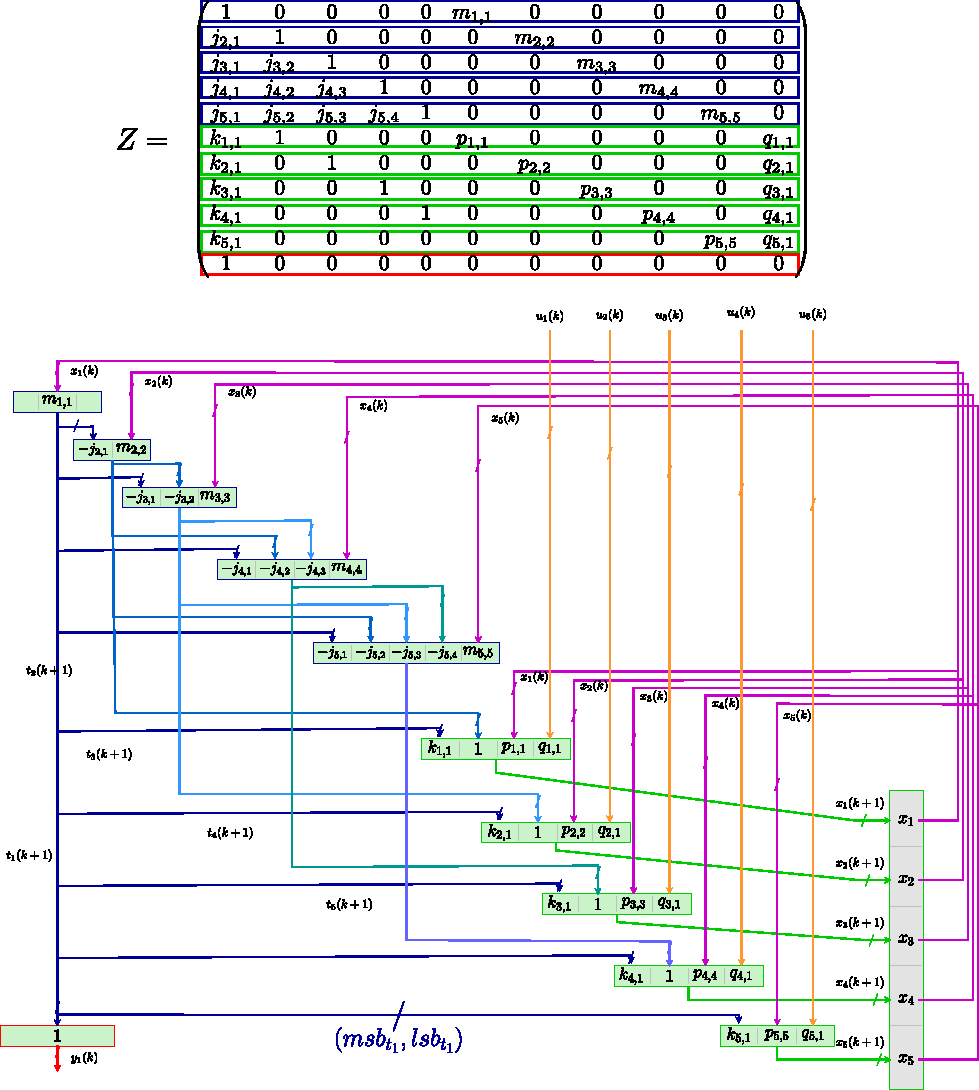
\includegraphics[scale=0.4]{pictures/exampleGreenFull.pdf}
	\end{figure}
\end{frame}

\begin{frame}
	\frametitle{Example}
	\begin{figure}
	  \begin{tikzpicture}

		%\normalsize 
		\footnotesize
		\node[draw, blue!100, thick, rectangle, minimum width =6.5cm, minimum height=0.25cm] (sel1)  at (5,9.1) {} ;
		\node[draw, blue1!100, thick, rectangle, minimum width =6.5cm, minimum height=0.25cm] (sel2)  at (5,7.2) {} ;
		\node[draw, blue2!100, thick, rectangle, minimum width =6.5cm, minimum height=0.25cm] (sel3)  at (5,5.4) {} ;
		\node[draw, blue3!100, thick, rectangle, minimum width =6.5cm, minimum height=0.25cm] (sel4)  at (5,3.6) {} ;
		\node[draw, blue4!100, thick, rectangle, minimum width =6.5cm, minimum height=0.25cm] (sel5)  at (5,1.8) {} ;
		\node[draw, green!100, thick, rectangle, minimum width =6.5cm, minimum height=0.25cm] (sel6)  at (5,0.0) {} ;
		\node[draw, green!100, thick, rectangle, minimum width =6.5cm, minimum height=0.25cm] (sel7)  at (5,-1.8) {} ;
		\node[draw, green!100, thick, rectangle, minimum width =6.5cm, minimum height=0.25cm] (sel8)  at (5,-3.6) {} ;
		\node[draw, green!100, thick, rectangle, minimum width =6.5cm, minimum height=0.25cm] (sel9)  at (5,-5.4) {} ;
		\node[draw, green!100, thick, rectangle, minimum width =6.5cm, minimum height=0.25cm] (sel10) at (5,-7.2) {} ;
		\node[draw, red!100, thick, rectangle, minimum width =6.5cm, minimum height=0.25cm] (sel11) at (5,-9.0) {} ;

		\node at (-20, 0) { \huge $Z = $};
		\normalsize
	  \node at (5, 0) {
		\resizebox{200pt}{!}{
			$\begin{pmatrix}
				1       & 0       & 0       & 0       & 0       & \textcolor{purple}{m_{1,1}} & 0       & 0       & 0       & 0       & 0       \\
				j_{2,1} & 1       & 0       & 0       & 0       & 0       & \textcolor{purple}{m_{2,2}} & 0       & 0       & 0       & 0       \\
				j_{3,1} & j_{3,2} & 1       & 0       & 0       & 0       & 0       & \textcolor{purple}{m_{3,3}} & 0       & 0       & 0       \\
				j_{4,1} & j_{4,2} & j_{4,3} & 1       & 0       & 0       & 0       & 0       & \textcolor{purple}{m_{4,4}} & 0       & 0       \\
				j_{5,1} & j_{5,2} & j_{5,3} & j_{5,4} & 1       & 0       & 0       & 0       & 0       & \textcolor{purple}{m_{5,5}} & 0       \\
				k_{1,1} & 1       & 0       & 0       & 0       & \textcolor{purple}{p_{1,1}} & 0       & 0       & 0       & 0       & \textcolor{orange}{q_{1,1}} \\

				k_{2,1} & 0       & 1       & 0       & 0       & 0       & \textcolor{purple}{p_{2,2}} & 0       & 0       & 0       & \textcolor{orange}{q_{2,1}} \\
				k_{3,1} & 0       & 0       & 1       & 0       & 0       & 0       & \textcolor{purple}{p_{3,3}} & 0       & 0       & \textcolor{orange}{q_{3,1}} \\
				k_{4,1} & 0       & 0       & 0       & 1       & 0       & 0       & 0       & \textcolor{purple}{p_{4,4}} & 0       & \textcolor{orange}{q_{4,1}} \\
				k_{5,1} & 0       & 0       & 0       & 0       & 0       & 0       & 0       & 0       & \textcolor{purple}{p_{5,5}} & \textcolor{orange}{q_{5,1}} \\

				1	    & 0       & 0       & 0       & 0       & 0       & 0       & 0       & 0       & 0       & 0       \\
			\end{pmatrix}$
	  }
	  };

		\end{tikzpicture}
	\end{figure}
	\centering
	Each line will be a SOPC
\end{frame}


\begin{frame}
	\frametitle{Example}
	\begin{figure}
		%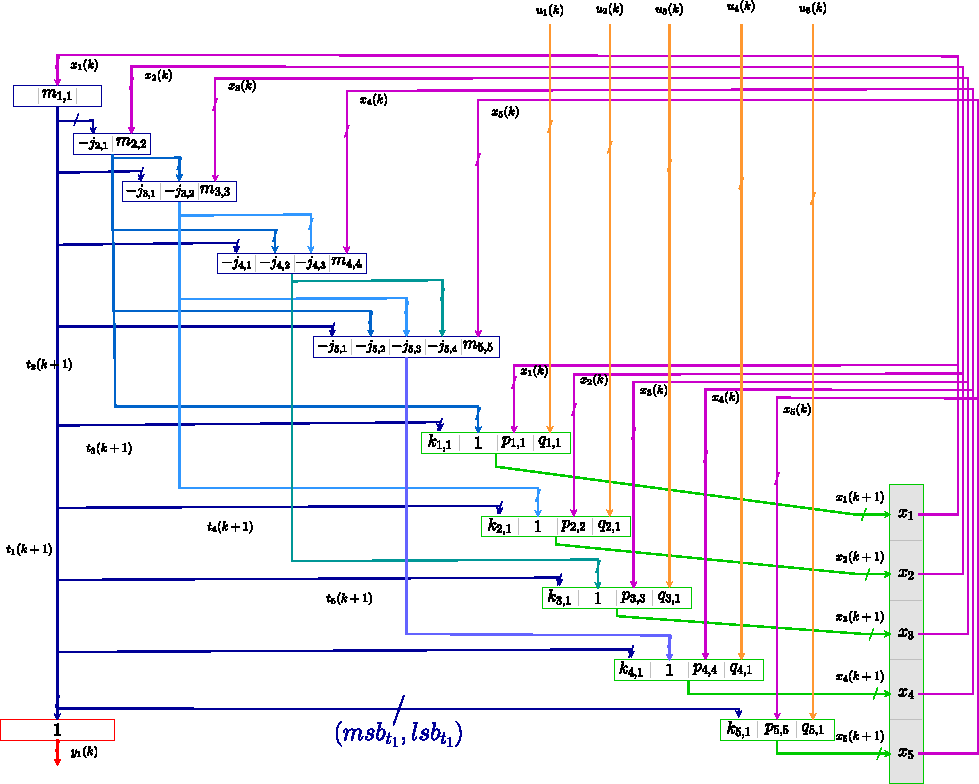
\includegraphics[scale=0.8]{pictures/exampleScheme.pdf}
		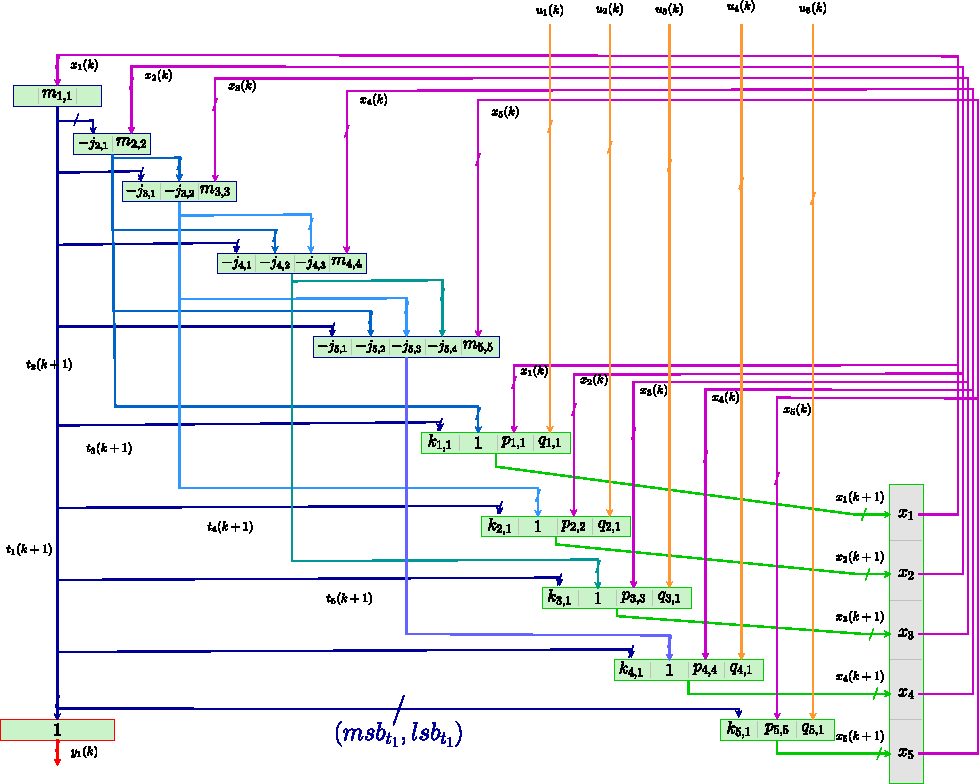
\includegraphics[scale=0.7, trim=0cm 5cm 2cm 0cm,clip]{pictures/exampleGreenScheme.pdf}
	\end{figure}
\end{frame}

\begin{frame}
	\frametitle{Example}
	\begin{figure}
		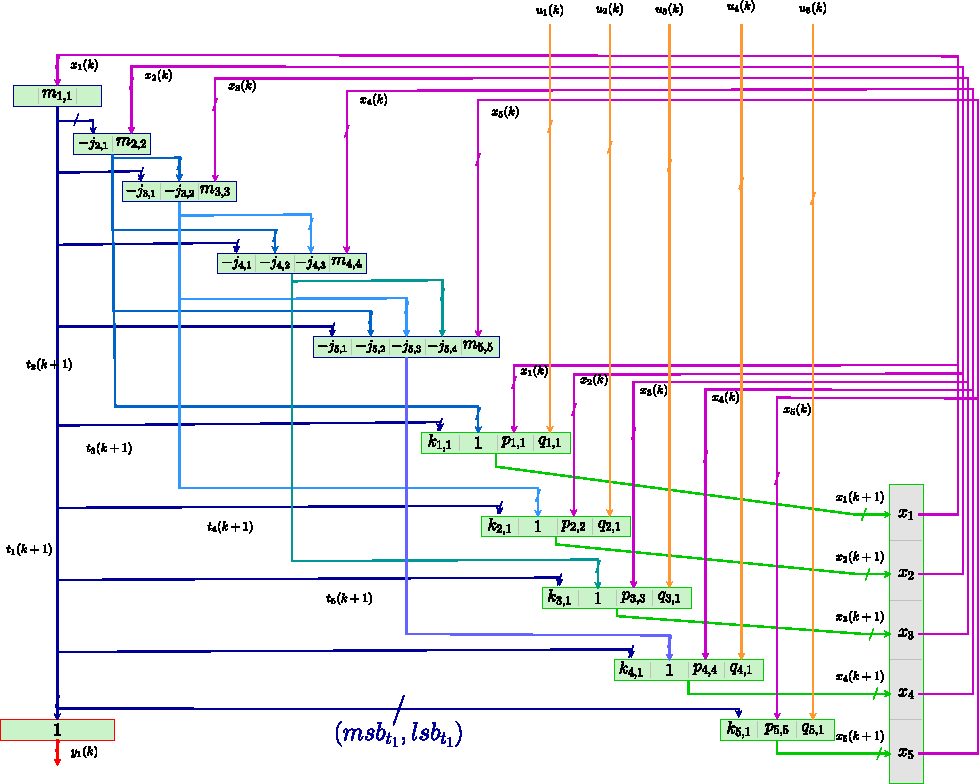
\includegraphics[scale=0.8, trim=5cm 0cm 0cm 5cm,clip]{pictures/exampleGreenScheme.pdf}
	\end{figure}
\end{frame}

\section{Computing the parameters}

\subsection{Computing the MSB}
\begin{frame}
	\frametitle{Computing the MSB}
	MSB should allow the full range of the signal.\\
	Worst-Case Peak Gain (WCPG):
	\begin{figure}
	\begin{tikzpicture}[domain=0:7.5, samples=1000]
		\draw[->] (-0.2,0) -- (10.2,0) node[right] {\tiny$k$};
		\draw[->] (0,-1.2) -- (0,7.2) node[above] {};
		\draw[<->] (3,-4.5) -- (3,5.5) node[above] {};
		\draw[-,dotted] (0.2,5.5) -- (3,5.5) node[right, yshift=2mm, xshift=-4mm] {\tiny $\|u\|_{l^\infty}$};
		\draw[-,dotted] (3,-4.5) -- (6,-4.5) node[above] {};
		\draw[color=blue] plot[id=sin] function{sin(x)+sin(2*x)+sin(3*x)+sin(4*x)+sin(5*x)+sin(6*x)+sin(7*x) * sin(8*x) +sin(9*x) *sin(10*x)} node[right] {\tiny$u(k)$};
		\draw (3.8cm,-0.3cm) -- (5.8cm,-0.3cm) [->, thick] node[above,near end]{};
		\draw (0.3cm,-0.3cm) -- (2.3cm,-0.3cm) [->, thick] node[above,near end]{};
		\draw (2.3cm,-0.8cm) rectangle ++ (1.5cm,1cm)[thick] node [midway]{$\mathcal{H}$}; 
		\draw[->] (23.8,1) -- (33.8,1) node[right] {\tiny$k$};
		\draw[->] (24,0.2) -- (24,8.2) node[above] {};
		\draw[<->] (27,-1.0) -- (27,3.0) node[above] {};
		\draw[-,dotted] (27,-1.0) -- (29,-1.0) node[right, yshift=9mm, xshift=-7mm] {\tiny $\|h * u\|_{l^\infty}$};
		\draw[-,dotted] (27,3.0) -- (26,3.0) node[above] {};
		\draw[color=red, xshift=117] plot[id=out] function{1+2*sin(x)} node[right] {\tiny$y(k)$};
	\end{tikzpicture}
	\end{figure}
	\begin{equation}
		\|\mathcal{H}\|_{wcpg}=\sup_{u\neq0}\frac{\|h*u\|_{l^{\infty}}}{\|u\|_{l^{\infty}}}
	\end{equation}
	\centering
	This computation is done by colleagues in LIP6.
\end{frame}

\subsection{Computing the LSB}

\begin{frame}
	$\boldsymbol{\varepsilon}$ is the error introduced by the SOPC (closely related to $2^{lsb_i}$). \\
	$\boldsymbol{\varepsilon^*}$ is the total error (taking the loopback into account)

	\frametitle{Computing the LSB: Point of view about error}
			\begin{figure}[h] 
			  \centering
			  \begin{tikzpicture}[x=1cm,y=1cm]
				\draw (-9, 0.5) -- (-8,0.5) [->, thick] node[above,near start]{$\boldsymbol{u}(k)$};
				\draw (-7.2, 1.5) -- (-7.2,1.0) [->, thick] node[right,near start]{$\boldsymbol{\varepsilon}(k)$};
				\draw (-6.5, 0.5) -- (-5.5,0.5) [->, thick] node[above,near end]{$\boldsymbol{y}^*(k)$};
				\draw (-8,0.0) rectangle ++(1.5,1)[thick] node [midway]{$\mathcal{H}$}; 
				\draw (-2,0.5) rectangle ++(1.5,1)[thick] node [midway]{$\mathcal{H}$}; 
				\draw (-3, 1) -- (-2,1) [->, thick] node [above,near start]{$\boldsymbol{u}(k)$}; 
				\draw (-0.5, 1)  -- (1,1) -- (1,0.5) [->, thick] node[xshift=-0.75cm,yshift=0.8cm]{$\boldsymbol{y}(k)$}; 

				\only<1>{\draw (-2,-1) rectangle ++(1.5,1)[thick] node [midway]{$\mathcal{H}_{\abserr}$}; }
				\only<2>{\draw (-2,-1) rectangle ++(1.5,1)[thick, fill=red!20] node [midway]{$\mathcal{H}_{\abserr}$}; }
				\draw (-3, -0.5) -- (-2,-0.5) [->, thick] node[above,near start]{$\boldsymbol{\varepsilon}(k)$};
				\draw (-0.5, -0.5) -- (1,-0.5) -- (1,0) [->, thick] node [xshift=-0.75cm,yshift=-0.2cm]{$\boldsymbol{\varepsilon^*_y}(k)$}; 

				\draw (1,0.25) circle (0.25) [thick] node {$+$}; 
				\draw (1.25,0.25) -- (2.25,0.25)[->, thick] node [above,midway] {$\boldsymbol{y}^*(k)$};

				\node (arrow) at (-4.3,0.4) {$\iff$};
			  \end{tikzpicture}

			%\caption{A signal view of the error propagation with respect to the ideal filter \label{fig:ltierror}}
			Error propagation with respect to the ideal filter
			\end{figure}
\end{frame}

\begin{frame}
	\frametitle{Computing the LSB: Impact of errors}
	\begin{algorithm}[H]
		\For{int i = 0 ; $i \leq n_t$; i++}{
			$\boldsymbol{t}_i(k+1) \leftarrow - \sum\limits\limits_{j<i} \boldsymbol{J}_{ij}\boldsymbol{t}_j(k+1) + \sum\limits_{j=1}^{n_x} \boldsymbol{M}_{ij}\boldsymbol{x}_j(k) + \sum\limits_{j=1}^{n_u} \boldsymbol{N}_{ij}\boldsymbol{u}_j(k) + \textcolor{red!80!gray}{\boldsymbol{\varepsilon}_{t_i}(k)}$
		}
		\For{int i = 0 ; $i \leq n_x$; i++}{
			$\boldsymbol{x}_i(k+1) \leftarrow \sum\limits_{j=1}^{n_t} \boldsymbol{K}_{ij}\boldsymbol{t}_j(k+1) + \sum\limits_{j=1}^{n_x} \boldsymbol{P}_{ij}\boldsymbol{x}_j(k) + \sum\limits_{j=1}^{n_u} \boldsymbol{Q}_{ij}\boldsymbol{u}_j(k) + \textcolor{red!80!gray}{\boldsymbol{\varepsilon}_{x_i}(k)}$
		}
		\For{int i = 0 ; $i \leq ny$; i++}{
			$\boldsymbol{y}_i(k) \leftarrow \sum\limits_{j=1}^{n_t} \boldsymbol{L}_{ij}\boldsymbol{t}_j(k+1) + \sum\limits_{j=1}^{n_x} \boldsymbol{R}_{ij}\boldsymbol{x}_j(k) + \sum\limits_{j=1}^{n_u} \boldsymbol{S}_{ij}\boldsymbol{u}_j(k) + \textcolor{red!80!gray}{\boldsymbol{\varepsilon}_{y_i}(k)}$
		}
		\caption{Computation of SIF outputs from inputs}
	\end{algorithm}
\end{frame}


\begin{frame}
	%3 dernières équations de calcul (avec le WCPG)
	\frametitle{Computing the LSB: current solution}
	Let's define:% $v'= n_t + n_x + n_y$ \\
			\begin{equation}
				\tiny
				\boldsymbol{v'}=
				\begin{pmatrix}
					\boldsymbol{t}(k+1) \\
					\boldsymbol{x}(k+1) \\
					\boldsymbol{y}(k)   \\
				\end{pmatrix}
			\end{equation}
	Main constraint:
		\begin{equation} \label{constraint}
			\boldsymbol{\varepsilon}_{v'} < \boldsymbol{2}^{-lsb_{v'}}
			%\boldsymbol{D} \cdot \boldsymbol{2}^{lsb_{v'}-msb_{v'}-1} < \boldsymbol{1}_{n_y}
		\end{equation}

	Transformed into the following constraint:

		\begin{equation} \label{constraint}
			| \langle\langle \mathcal{H}_{\boldsymbol{\varepsilon}} \rangle\rangle_{} | \cdot \boldsymbol{2}^{lsb_{v'}+1} < \boldsymbol{2}^{-lsb_{y_i}}
			%\boldsymbol{D} \cdot \boldsymbol{2}^{lsb_{v'}-msb_{v'}-1} < \boldsymbol{1}_{n_y}
		\end{equation}
	%Then: constraint on each line of the computation algorithm.
	Lopez gives a simple solution that matches the fixed size constraint.\\
	The solution matching the hardware context (arbitrary precision) is work in progress.

%		\begin{eqnarray}
%			\boldsymbol{\mathfrak{A}}_{i,j}= | \langle\langle \mathcal{H}_{\boldsymbol{\varepsilon}} \rangle\rangle_{i,j} | \cdot \frac{\boldsymbol{2^{msb_{v'_j}+1}}}{\xi_i} %\\
%			%\boldsymbol{D}_{i,j}= | \langle\langle \mathcal{H}_{\boldsymbol{\varepsilon}} \rangle\rangle_{i,j}| \cdot \frac{\boldsymbol{2^{msb_{v'_j}+1}}}{\xi_i}
%		\end{eqnarray}
\end{frame}

